% Optimizing CF-LIBS Element Identification:
% From LLM-Driven Code Evolution to GPU-Accelerated CMA-ES
% Beamer presentation — full experimental campaign
\documentclass[aspectratio=169,12pt]{beamer}

% --- Theme and colors ---
\usetheme{metropolis}
\usepackage{appendixnumberbeamer}

% Colorblind-safe palette (same as paper)
\definecolor{cbBlue}{HTML}{0072B2}
\definecolor{cbOrange}{HTML}{D55E00}
\definecolor{cbGreen}{HTML}{009E73}
\definecolor{cbYellow}{HTML}{F0E442}
\definecolor{cbPurple}{HTML}{CC79A7}

\setbeamercolor{frametitle}{bg=cbBlue,fg=white}
\setbeamercolor{progress bar}{fg=cbOrange}
\setbeamercolor{alerted text}{fg=cbOrange}

% --- Packages ---
\usepackage{amsmath,amssymb}
\usepackage{graphicx}
\usepackage{booktabs}
\usepackage{siunitx}
\usepackage{bm}
\usepackage{tikz}
\usepackage{multicol}

\usetikzlibrary{arrows.meta,positioning,calc,fit,shapes.geometric}

\sisetup{
  separate-uncertainty = true,
  multi-part-units = single,
}

% --- Metadata ---
\title{Optimizing CF-LIBS Element Identification}
\subtitle{From LLM Code Evolution to GPU CMA-ES --- A 7-Order-of-Magnitude Speedup}
\author{Brian Squires}
\institute{[Affiliation]}
\date{2026}

% ============================================================
\begin{document}

% ----------------------------------------------------------
% SLIDE 1: Title
% ----------------------------------------------------------
\begin{frame}[plain]
  \titlepage
\note{
  Good morning. I will present our experimental campaign to optimize
  the element identification pipeline in CF-LIBS. We explored three
  optimization approaches --- LLM-driven code evolution, GPU-accelerated
  CMA-ES on threshold parameters, and finally a 101-parameter separable
  CMA-ES across all five identification algorithms. The final result:
  F-beta of 0.914, a 7-order-of-magnitude speedup in evaluations per second,
  and physically interpretable optimized parameters.
}
\end{frame}

% ----------------------------------------------------------
% SLIDE 2: The Element ID Challenge
% ----------------------------------------------------------
\begin{frame}{The Element Identification Challenge}
  \begin{columns}[T]
    \begin{column}{0.55\textwidth}
      \textbf{CF-LIBS requires knowing which elements are present}
      \begin{itemize}
        \item Must identify elements \emph{before} quantification
        \item At RP $< 1000$: severe spectral overlap
        \item Line blending, chance coincidences, dense forests
        \item Mn: $>500$ transitions create pseudo-continuum
      \end{itemize}

      \vspace{0.8em}
      \textbf{The combiner function:}
      \begin{itemize}
        \item Fuses scores from identification algorithms
        \item Traditionally hand-tuned (geometric mean + thresholds)
        \item \alert{Can we optimize this automatically?}
      \end{itemize}
    \end{column}
    \begin{column}{0.42\textwidth}
      \centering
      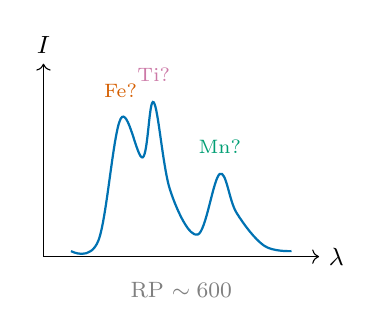
\begin{tikzpicture}[scale=0.7, every node/.style={font=\small}]
        % Spectrum sketch
        \draw[->] (0,0) -- (5,0) node[right] {$\lambda$};
        \draw[->] (0,0) -- (0,3.5) node[above] {$I$};
        % Overlapping peaks
        \draw[cbBlue, thick] plot[smooth, tension=0.6] coordinates
          {(0.5,0.1) (1.0,0.3) (1.4,2.5) (1.8,1.8) (2.0,2.8)
           (2.3,1.2) (2.8,0.4) (3.2,1.5) (3.5,0.8) (4.0,0.2) (4.5,0.1)};
        % Labels
        \node[cbOrange, font=\scriptsize] at (1.4,3.0) {Fe?};
        \node[cbPurple, font=\scriptsize] at (2.0,3.3) {Ti?};
        \node[cbGreen, font=\scriptsize] at (3.2,2.0) {Mn?};
        % RP annotation
        \node[font=\footnotesize, text=gray] at (2.5,-0.6) {RP $\sim 600$};
      \end{tikzpicture}
    \end{column}
  \end{columns}
\note{
  CF-LIBS works backwards from emission spectra to composition.
  But first you must identify which elements are present.
  At low resolving power, peaks overlap badly --- manganese alone
  has over 500 transitions that create a pseudo-continuum.
  The combiner function that fuses identification scores is traditionally
  hand-tuned. Our question: can we optimize it automatically?
}
\end{frame}

% ----------------------------------------------------------
% SLIDE 3: Baseline Performance (updated with teaser)
% ----------------------------------------------------------
\begin{frame}{Baseline Performance: Five Identification Pathways}
  {\small
  \begin{table}
    \centering
    \begin{tabular}{@{}llccc@{}}
      \toprule
      Rank & Pathway & P & R & F$_1$ \\
      \midrule
      1 & Hybrid NNLS+ALIAS & 0.604 & 0.713 & \alert{0.654} \\
      2 & ALIAS peak-matching & 0.505 & 0.629 & 0.560 \\
      3 & Voigt + ALIAS & 0.488 & 0.623 & 0.547 \\
      4 & Forward model & 0.369 & 0.796 & 0.505 \\
      5 & Spectral NNLS & 0.293 & 0.940 & 0.447 \\
      \bottomrule
    \end{tabular}
  \end{table}
  }

  \vspace{0.3em}
  \begin{itemize}
    \item 74 Aalto mineral spectra, RP = 300--1100
    \item Best hand-tuned: Hybrid at F$_1 = 0.654$
    \item Even the best pathway misidentifies $>$30\% of elements
    \item \alert{Spoiler:} by the end of this talk, we reach \alert{F$_\beta = 0.914$}
  \end{itemize}
\note{
  Our benchmark evaluated five pathways on 74 real mineral spectra.
  The best hand-tuned approach, hybrid NNLS plus ALIAS, reaches F1 of 0.654.
  Even that misidentifies over 30 percent of elements.
  By the end of this talk we will reach F-beta of 0.914 through
  a progression of three increasingly powerful optimization approaches.
}
\end{frame}

% ----------------------------------------------------------
% SLIDE 4: Why Optimize the Combiner?
% ----------------------------------------------------------
\begin{frame}{Why Optimize the Combiner?}
  \begin{columns}[T]
    \begin{column}{0.48\textwidth}
      \textbf{What the combiner does:}
      \begin{itemize}
        \item Receives per-element scores from each algorithm
        \item \texttt{score}, \texttt{n\_matched}, \texttt{SNR}, \texttt{confidence}
        \item Decides: detected or not?
      \end{itemize}

      \vspace{0.5em}
      \textbf{Hand-tuned baseline:}
      \begin{itemize}
        \item Geometric mean + AND gate
        \item Fixed global threshold (0.30)
        \item Single operating point
      \end{itemize}
    \end{column}
    \begin{column}{0.48\textwidth}
      \textbf{The optimization opportunity:}
      \begin{itemize}
        \item The combiner is a \emph{function} over scores
        \item Huge design space: weighting, thresholds, gating logic
        \item Per-element, per-algorithm behavior possible
        \item \alert{Goal:} discover better strategies automatically
      \end{itemize}

      \vspace{0.5em}
      \begin{block}{Key insight}
        The combiner is the cheapest place to improve ---
        no new physics, no new hardware, just better scoring.
      \end{block}
    \end{column}
  \end{columns}
\note{
  The combiner function takes per-element scores from each algorithm and decides
  which elements to report as detected. The hand-tuned version uses
  a geometric mean with a fixed threshold of 0.30. But this is really a function
  optimization problem with a huge design space. And it is the cheapest
  place to improve: no new hardware, no new physics, just better logic.
}
\end{frame}

% ----------------------------------------------------------
% SLIDE 5: Three Optimization Approaches (NEW - replaces MAP-Elites)
% ----------------------------------------------------------
\begin{frame}{Three Optimization Approaches}
  \centering
  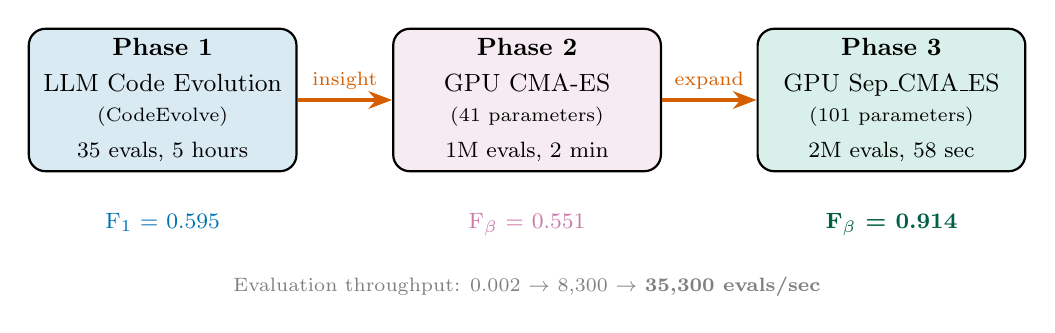
\begin{tikzpicture}[
    node distance=0.4cm and 0.8cm,
    box/.style={draw, rounded corners=6pt, minimum width=3.4cm,
                minimum height=1.6cm, font=\small, align=center, thick},
    arr/.style={-{Stealth[length=3mm]}, very thick, cbOrange},
    every node/.style={font=\small}
  ]
    \node[box, fill=cbBlue!15] (ce) {
      \textbf{Phase 1}\\[2pt]
      LLM Code Evolution\\
      {\scriptsize (CodeEvolve)}\\[2pt]
      {\footnotesize 35 evals, 5 hours}
    };
    \node[box, fill=cbPurple!15, right=1.2cm of ce] (cma41) {
      \textbf{Phase 2}\\[2pt]
      GPU CMA-ES\\
      {\scriptsize (41 parameters)}\\[2pt]
      {\footnotesize 1M evals, 2 min}
    };
    \node[box, fill=cbGreen!15, right=1.2cm of cma41] (cma101) {
      \textbf{Phase 3}\\[2pt]
      GPU Sep\_CMA\_ES\\
      {\scriptsize (101 parameters)}\\[2pt]
      {\footnotesize 2M evals, 58 sec}
    };

    \draw[arr] (ce) -- node[above, font=\scriptsize] {insight} (cma41);
    \draw[arr] (cma41) -- node[above, font=\scriptsize] {expand} (cma101);

    % Results below
    \node[font=\footnotesize, cbBlue, below=0.4cm of ce] {F$_1$ = 0.595};
    \node[font=\footnotesize, cbPurple, below=0.4cm of cma41] {F$_\beta$ = 0.551};
    \node[font=\footnotesize, cbGreen!60!black, below=0.4cm of cma101, font=\footnotesize\bfseries] {F$_\beta$ = 0.914};

    % Speed annotation
    \node[font=\scriptsize, text=gray, below=1.2cm of cma41]
      {Evaluation throughput: 0.002 $\to$ 8{,}300 $\to$ \textbf{35{,}300 evals/sec}};
  \end{tikzpicture}
\note{
  Our experimental campaign progressed through three phases. Phase 1 used
  LLMs as mutation operators to evolve combiner code --- slow but produced
  physically interpretable innovations. Phase 2 moved to GPU-accelerated
  CMA-ES on 41 continuous threshold parameters, achieving a million evaluations
  in two minutes. Phase 3 expanded to 101 parameters across all five algorithms
  using separable CMA-ES, reaching F-beta of 0.914. Evaluation throughput
  increased by seven orders of magnitude across the campaign.
}
\end{frame}

% ----------------------------------------------------------
% SLIDE 6: LLM-as-Mutation-Operator (Phase 1 intro)
% ----------------------------------------------------------
\begin{frame}{Phase 1: LLM-as-Mutation-Operator}
  \begin{columns}[T]
    \begin{column}{0.50\textwidth}
      \textbf{Traditional genetic programming:}
      \begin{itemize}
        \item Syntax-tree crossover/mutation
        \item Brittle, slow convergence
        \item No domain awareness
      \end{itemize}

      \vspace{0.8em}
      \textbf{Our approach:}
      \begin{itemize}
        \item LLM receives parent code + fitness metrics
        \item Generates \emph{semantically meaningful} variant
        \item Understands atomic physics context
        \item ``Add element-specific threshold for Na''\\
              vs random subtree swap
      \end{itemize}
    \end{column}
    \begin{column}{0.47\textwidth}
      \centering
      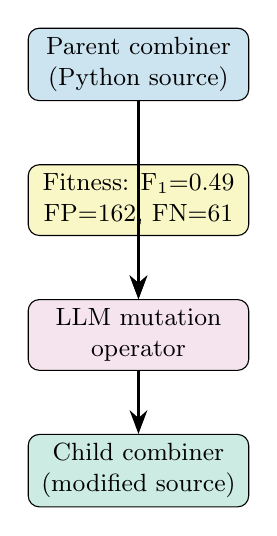
\begin{tikzpicture}[
        node distance=0.8cm,
        box/.style={draw, rounded corners, minimum width=2.8cm,
                    minimum height=0.7cm, font=\small, align=center},
        arr/.style={-{Stealth[length=3mm]}, thick}
      ]
        \node[box, fill=cbBlue!20] (parent) {Parent combiner\\(Python source)};
        \node[box, fill=cbYellow!30, below=of parent] (metrics) {Fitness: F$_1$=0.49\\FP=162, FN=61};
        \node[box, fill=cbPurple!20, below=of metrics] (llm) {LLM mutation\\operator};
        \node[box, fill=cbGreen!20, below=of llm] (child) {Child combiner\\(modified source)};

        \draw[arr] (parent) -- (llm);
        \draw[arr] (metrics) -- (llm);
        \draw[arr] (llm) -- (child);
      \end{tikzpicture}

      \vspace{0.5em}
      {\footnotesize 6 models: Opus, Sonnet, Gemini,\\GPT-5.4, 122B, 80B local}
    \end{column}
  \end{columns}
\note{
  Phase 1 used large language models as the mutation operator in a MAP-Elites
  quality-diversity search. The LLMs receive the parent combiner code plus
  its fitness metrics and produce semantically meaningful variants. This is
  fundamentally different from random syntax-tree mutation: the LLM understands
  the domain and can propose targeted changes like ``add a threshold for sodium.''
  We used six models spanning cloud and local HPC.
}
\end{frame}

% ----------------------------------------------------------
% SLIDE 7: Multi-Model Ensemble
% ----------------------------------------------------------
\begin{frame}{Phase 1: Multi-Model Ensemble}
  \begin{columns}[T]
    \begin{column}{0.52\textwidth}
      {\small
      \begin{table}
        \centering
        \begin{tabular}{@{}lccc@{}}
          \toprule
          Model & Median & P90 & Success \\
          \midrule
          Sonnet 4.6 & 56s & 84s & \alert{100\%} \\
          Opus 4.6 & 60s & 90s & 100\% \\
          Gemini 3.1 Pro & 164s & 260s & 100\% \\
          GPT-5.4 & 238s & 277s & \textcolor{red}{0\%} \\
          \rowcolor{cbBlue!10}
          27B Scout & 264s & 515s & 33\% \\
          \rowcolor{cbBlue!10}
          122B Coder & 322s & 2188s & 40\% \\
          \bottomrule
        \end{tabular}
      \end{table}
      }
      {\scriptsize N = 109 calls across all runs}
    \end{column}
    \begin{column}{0.45\textwidth}
      \textbf{Key findings:}
      \begin{itemize}
        \item \alert{Sonnet > Opus > Gemini}\\
              for this task
        \item GPT-5.4: completely broken\\
              (0\% success, 14 calls)
        \item Cloud models \textbf{5$\times$ faster}\\
              and \textbf{2.5$\times$ more reliable}\\
              than local
        \item 122B too slow for complex\\
              seed code ($>$35 min/call)
      \end{itemize}

      \vspace{0.3em}
      \begin{alertblock}{Lesson}
        LLMs are good \emph{innovators} but expensive \emph{optimizers}
      \end{alertblock}
    \end{column}
  \end{columns}
\note{
  Across 109 calls, Sonnet 4.6 was the most effective model: fastest median
  latency at 56 seconds with 100 percent success. Opus was a close second.
  GPT-5.4 was completely broken with zero percent success across 14 calls.
  Local models were 5x slower and far less reliable --- the 122B model
  took over 35 minutes per call on complex seed code. The key lesson:
  LLMs are good at discovering innovations but expensive as optimizers.
}
\end{frame}

% ----------------------------------------------------------
% SLIDE 8: Phase 1 Results
% ----------------------------------------------------------
\begin{frame}{Phase 1: CodeEvolve Results}
  \begin{columns}[T]
    \begin{column}{0.52\textwidth}
      {\small
      \begin{table}
        \centering
        \begin{tabular}{@{}lccc@{}}
          \toprule
          Metric & Baseline & Evolved & $\Delta$ \\
          \midrule
          F$_1$ & 0.487 & \alert{0.595} & \alert{+22\%} \\
          Precision & 0.396 & \alert{0.610} & \alert{+54\%} \\
          Recall & 0.635 & 0.581 & $-8$\% \\
          False Pos. & 162 & \alert{62} & \alert{$-62$\%} \\
          \bottomrule
        \end{tabular}
      \end{table}
      }

      \vspace{0.3em}
      {\small Island 2, Epoch 9 of 23\\
       Best of only \alert{35 total evaluations}\\
       ALIAS-only features (no NNLS)}
    \end{column}
    \begin{column}{0.45\textwidth}
      \textbf{The recall bias problem:}\\
      LLMs consistently evolve toward\\
      ``detect more'' rather than\\
      ``reject false positives''

      \vspace{0.5em}
      {\small
      \begin{itemize}
        \item F$_1$ creates asymmetric gradient\\
              favoring recall
        \item Run 2a (NNLS+ALIAS):\\
              R=0.74 but P=0.43
        \item F$_\beta$(0.5) intervention helped\\
              but couldn't break through
      \end{itemize}
      }

      \vspace{0.3em}
      \begin{block}{Insight}
        LLMs discover \emph{strategies};\\
        CMA-ES optimizes \emph{parameters}
      \end{block}
    \end{column}
  \end{columns}
\note{
  CodeEvolve Run 1 improved F1 by 22 percent and cut false positives by 62 percent
  in just 35 evaluations. But we hit a fundamental limitation: LLMs have a recall bias.
  They consistently evolve code that detects more elements rather than rejecting
  false positives. Switching to F-beta with precision weighting helped but couldn't
  overcome this. The key insight was that LLMs are good at discovering strategies ---
  but continuous parameter optimization should be done by a numerical optimizer.
}
\end{frame}

% ----------------------------------------------------------
% SLIDE 9: What the Evolved Combiner Discovered (kept)
% ----------------------------------------------------------
\begin{frame}{Phase 1: What the LLM Discovered}
  \begin{columns}[T]
    \begin{column}{0.50\textwidth}
      \textbf{9 physics-grounded innovations:}
      \begin{enumerate}
        \item Element-specific thresholds\\
              {\scriptsize (Na=0.42, K=0.44, Mn=0.46)}
        \item Line credibility factor\\
              {\scriptsize ($n_\mathrm{matched}=0 \to$ veto)}
        \item SNR sigmoid weighting\\
              {\scriptsize ($\sigma(1.5 \cdot (\mathrm{SNR}-2.5))$)}
        \item Power mean combination ($p=-0.5$)
        \item Dual-detector agreement bonus
      \end{enumerate}
    \end{column}
    \begin{column}{0.47\textwidth}
      \begin{enumerate}\setcounter{enumi}{5}
        \item Percentile-rank context (28\% weight)
        \item Adaptive threshold adjustment
        \item Multi-stage rescue logic
        \item Anti-false-positive vetoes
      \end{enumerate}

      \vspace{0.5em}
      \begin{exampleblock}{Key value of Phase 1}
        Every innovation is \emph{physically interpretable} ---
        encodes domain knowledge that spectroscopists use intuitively.
        No black boxes.
      \end{exampleblock}

      \vspace{0.3em}
      {\scriptsize These strategies informed the\\
       parameter space design for Phase 2.}
    \end{column}
  \end{columns}
\note{
  The LLM's greatest contribution was not the F1 score but the innovations themselves.
  Nine distinct strategies, all physics-grounded: element-specific thresholds based
  on known false-positive behavior, an SNR sigmoid centered at the IUPAC detection limit,
  line credibility weighting, dual-detector agreement bonuses. These innovations
  encode domain knowledge that spectroscopists use intuitively. Crucially, they
  informed the parameter space design for the GPU CMA-ES phase that followed.
}
\end{frame}

% ----------------------------------------------------------
% SLIDE 10: Transition to CMA-ES
% ----------------------------------------------------------
\begin{frame}{The Transition: From LLM to CMA-ES}
  \begin{columns}[T]
    \begin{column}{0.50\textwidth}
      \textbf{Why switch from LLMs?}
      \begin{itemize}
        \item LLM mutations: $\sim$0.002 evals/sec
        \item Recall bias in code generation
        \item 122B model: 35 min per call\\
              on complex seed code
        \item F$_1$ plateaued at 0.595
      \end{itemize}

      \vspace{0.5em}
      \textbf{The insight:}\\
      The LLMs discovered \emph{what parameters matter}\\
      (thresholds, SNR gates, per-element tuning).

      \vspace{0.3em}
      Now let a numerical optimizer find\\
      \emph{the optimal values}.
    \end{column}
    \begin{column}{0.47\textwidth}
      \textbf{GPU CMA-ES design:}
      \begin{itemize}
        \item Extract all tunable parameters\\
              into a continuous vector
        \item Vectorize evaluation on GPU\\
              (JAX + cached algorithm outputs)
        \item CMA-ES: derivative-free,\\
              population-based, robust
      \end{itemize}

      \vspace{0.5em}
      \textbf{Phase 2: 41 parameters}\\
      {\small Single-algorithm thresholds + SNR + scoring}

      \vspace{0.3em}
      \textbf{Phase 3: 101 parameters}\\
      {\small All 5 algorithms + per-element + fusion}

      \vspace{0.3em}
      {\small Hardware: V100S GPUs (same HPC cluster)}
    \end{column}
  \end{columns}
\note{
  The transition from LLMs to CMA-ES was motivated by three problems:
  slow evaluation rate at 0.002 evals per second, the recall bias in
  LLM-generated code, and plateauing F1. But the LLMs gave us the crucial
  insight: what parameters matter. Element-specific thresholds, SNR gates,
  per-element tuning --- these are the axes of the optimization landscape.
  We extracted 41 tunable parameters into a continuous vector and ran CMA-ES
  on GPU with vectorized evaluation using cached algorithm outputs.
}
\end{frame}

% ----------------------------------------------------------
% SLIDE 11: CMA-ES 41-param Results (Phase 2)
% ----------------------------------------------------------
\begin{frame}{Phase 2: GPU CMA-ES --- 41 Parameters}
  \begin{columns}[T]
    \begin{column}{0.50\textwidth}
      \textbf{Configuration:}
      \begin{itemize}
        \item 41 continuous parameters\\
              {\scriptsize (thresholds, SNR gate, scoring weights)}
        \item 200 generations $\times$ 5{,}000 population
        \item \alert{1{,}000{,}000 evals in 2 minutes}
        \item Single V100S GPU
      \end{itemize}

      \vspace{0.5em}
      \textbf{Result:} F$_\beta$(0.5) = \alert{0.551}\\
      Converged by generation $\sim$15

      \vspace{0.3em}
      Multi-GPU (3$\times$V100S) confirmed:\\
      same optimum, 1.5M evals in 3 min
    \end{column}
    \begin{column}{0.47\textwidth}
      \textbf{Key parameter shifts:}
      {\small
      \begin{table}
        \begin{tabular}{@{}lcc@{}}
          \toprule
          Parameter & Base & Opt \\
          \midrule
          thresh\_default & 0.30 & \alert{0.90} \\
          SNR center & 2.5 & \alert{5.4} \\
          thresh\_K & 0.44 & 0.91 \\
          thresh\_Li & 0.40 & 0.92 \\
          rescue\_comb\_min & 0.60 & 0.93 \\
          \bottomrule
        \end{tabular}
      \end{table}
      }

      \vspace{0.3em}
      \begin{alertblock}{Physical insight}
        The baseline was \emph{far too permissive}.\\
        Default threshold: 0.30 $\to$ 0.90.\\
        SNR gate: below IUPAC 3$\sigma$ $\to$ well above.
      \end{alertblock}
    \end{column}
  \end{columns}
\note{
  Phase 2 ran CMA-ES on 41 continuous parameters: thresholds, SNR gates,
  and scoring weights for the single ALIAS algorithm. One million evaluations
  in two minutes on a single V100S. The result: F-beta of 0.551.
  The most dramatic finding was that the baseline thresholds were far too
  permissive. The default threshold jumped from 0.30 to 0.90 --- you need
  90 percent confidence to be detected. The SNR center moved from 2.5 to 5.4,
  well above the IUPAC 3-sigma detection limit. Multi-GPU confirmed this
  is the global optimum for the 41-parameter space.
}
\end{frame}

% ----------------------------------------------------------
% SLIDE 12: Phase 2 Gradient Analysis
% ----------------------------------------------------------
\begin{frame}{Phase 2: Gradient Analysis --- The Optimization Landscape}
  \begin{columns}[T]
    \begin{column}{0.50\textwidth}
      \textbf{Most sensitive dimensions over time:}

      \vspace{0.3em}
      {\small
      \begin{table}
        \begin{tabular}{@{}clc@{}}
          \toprule
          Gen & Dimension & $|\nabla|$ \\
          \midrule
          \multirow{2}{*}{0} & thresh\_default & 0.090 \\
          & veto\_alias\_min & 0.021 \\
          \midrule
          \multirow{2}{*}{10} & snr\_center & 0.045 \\
          & snr\_steepness & 0.029 \\
          \midrule
          40+ & all & $<$0.006 \\
          \bottomrule
        \end{tabular}
      \end{table}
      }

      \vspace{0.3em}
      Flat landscape after gen 40:\\
      \alert{global optimum reached}
    \end{column}
    \begin{column}{0.47\textwidth}
      \textbf{Interpretation:}
      \begin{itemize}
        \item Gen 0--10: threshold correction\\
              dominates (biggest gain from\\
              raising the detection bar)
        \item Gen 10--30: SNR gate\\
              fine-tuning (second-order\\
              precision improvements)
        \item Gen 40+: exhausted ---\\
              no more gains possible\\
              in 41-dim space
      \end{itemize}

      \vspace{0.5em}
      \begin{block}{Conclusion}
        F$_\beta$ = 0.551 is the \textbf{ceiling}\\
        for single-algorithm thresholds.\\
        Need to expand the search space.
      \end{block}
    \end{column}
  \end{columns}
\note{
  The gradient analysis tells us exactly how CMA-ES found the optimum.
  In the first 10 generations, the default threshold was the most sensitive
  dimension --- the biggest gain came from simply raising the detection bar.
  Then SNR gate tuning dominated from generation 10 to 30. After generation 40,
  all gradients fell below 0.006 --- the landscape was completely flat.
  F-beta 0.551 is the global optimum for the 41-parameter single-algorithm space.
  To go further, we needed to expand the search space to all five algorithms.
}
\end{frame}

% ----------------------------------------------------------
% SLIDE 13: Sep_CMA_ES 101-param Design (Phase 3)
% ----------------------------------------------------------
\begin{frame}{Phase 3: Full Ensemble Optimization --- 101 Parameters}
  \begin{columns}[T]
    \begin{column}{0.50\textwidth}
      \textbf{Parameter groups:}
      {\small
      \begin{table}
        \begin{tabular}{@{}lr@{}}
          \toprule
          Group & Params \\
          \midrule
          Algorithm selection (softmax) & 5 \\
          ALIAS identifier & 14 \\
          NNLS identifier & 5 \\
          Hybrid identifier & 13 \\
          Correlation identifier & 17 \\
          Comb identifier & 14 \\
          Per-element thresholds & 22 \\
          Decision fusion & 10 \\
          \midrule
          \textbf{Total} & \textbf{101} \\
          \bottomrule
        \end{tabular}
      \end{table}
      }
    \end{column}
    \begin{column}{0.47\textwidth}
      \textbf{Technical details:}
      \begin{itemize}
        \item Algorithm: evosax Sep\_CMA\_ES\\
              {\scriptsize (separable covariance --- avoids\\
               cuSolver bug on V100S)}
        \item Population: 4{,}096 per generation
        \item Generations: 500
        \item Hardware: single V100S
        \item Speed: $\sim$45{,}000 evals/sec
      \end{itemize}

      \vspace{0.3em}
      \textbf{Cache:} all 5 algorithm outputs\\
      on all 74 spectra (real physics)\\
      {\small ALIAS, NNLS, Hybrid, Correlation, Comb}

      \vspace{0.3em}
      \textbf{Fitness:} F$_\beta$(0.5)\\
      {\small (precision-weighted, 2$\times$ P over R)}
    \end{column}
  \end{columns}
\note{
  Phase 3 expanded from 41 to 101 parameters spanning all five identification
  algorithms. Five algorithm selection weights use softmax normalization.
  Each algorithm has its own tunable parameters. Twenty-two per-element thresholds
  allow element-specific detection decisions. Ten decision fusion parameters
  control how algorithm outputs are combined. We used evosax Sep-CMA-ES with
  separable covariance to avoid a cuSolver bug on V100S. Population of 4096,
  running 500 generations at 45,000 evaluations per second on a single GPU.
  The cache contains real physics outputs from all five algorithms on all 74 spectra.
}
\end{frame}

% ----------------------------------------------------------
% SLIDE 14: Sep_CMA_ES Convergence (Phase 3 results)
% ----------------------------------------------------------
\begin{frame}{Phase 3: Convergence --- 0.497 to 0.914}
  \begin{columns}[T]
    \begin{column}{0.52\textwidth}
      {\small
      \begin{table}
        \centering
        \begin{tabular}{@{}rrl@{}}
          \toprule
          Gen & F$_\beta$(0.5) & Notes \\
          \midrule
          0 & 0.497 & Baseline \\
          1 & 0.654 & Matches best hand-tuned \\
          4 & \alert{0.662} & Exceeds all hand-tuned \\
          20 & 0.751 & \\
          30 & 0.811 & \\
          70 & 0.855 & \\
          100 & 0.880 & \\
          150 & 0.896 & \\
          300 & \alert{\textbf{0.914}} & \textbf{Converged} \\
          \bottomrule
        \end{tabular}
      \end{table}
      }

      \vspace{0.3em}
      {\small 2{,}048{,}000 evaluations in \alert{58 seconds}}
    \end{column}
    \begin{column}{0.45\textwidth}
      \centering
      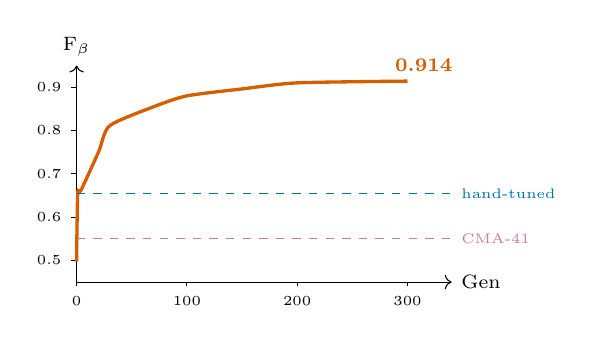
\begin{tikzpicture}[xscale=0.014, yscale=5.5]
        % Axes
        \draw[->] (0,0.45) -- (340,0.45) node[right, font=\scriptsize] {Gen};
        \draw[->] (0,0.45) -- (0,0.95) node[above, font=\scriptsize] {F$_\beta$};
        % Tick marks
        \foreach \x/\l in {0/0, 100/100, 200/200, 300/300} {
          \draw (\x,0.45) -- (\x,0.44) node[below, font=\tiny] {\l};
        }
        \foreach \y/\l in {0.5/0.5, 0.6/0.6, 0.7/0.7, 0.8/0.8, 0.9/0.9} {
          \draw (0,\y) -- (-5,\y) node[left, font=\tiny] {\l};
        }
        % Convergence curve
        \draw[cbOrange, very thick] plot[smooth, tension=0.4] coordinates {
          (0,0.497) (1,0.654) (4,0.662) (20,0.751) (30,0.811)
          (70,0.855) (100,0.880) (150,0.896) (200,0.910) (300,0.914)
        };
        % Horizontal reference lines
        \draw[cbBlue, dashed, thin] (0,0.654) -- (340,0.654)
          node[right, font=\tiny, cbBlue] {hand-tuned};
        \draw[cbPurple, dashed, thin] (0,0.551) -- (340,0.551)
          node[right, font=\tiny, cbPurple] {CMA-41};
        % Final point
        \fill[cbOrange] (300,0.914) circle (0.008);
        \node[above right, font=\scriptsize, cbOrange] at (280,0.914) {\textbf{0.914}};
      \end{tikzpicture}

      \vspace{0.3em}
      {\small Surpasses hand-tuned hybrid\\
       in \textbf{1 generation} (4{,}096 evals)}

      \vspace{0.3em}
      {\small Validated against real\\5-algorithm cache outputs}
    \end{column}
  \end{columns}
\note{
  The convergence curve tells a remarkable story. Generation 0 starts at
  F-beta 0.497. After just ONE generation --- 4,096 evaluations --- it matches
  the best hand-tuned hybrid at 0.654. By generation 4 it exceeds all
  hand-tuned results. The curve continues climbing through 0.811 at generation 30,
  0.880 at generation 100, and converges at 0.914 at generation 300.
  The entire optimization --- 2 million evaluations --- took 58 seconds
  on a single V100S GPU. This result is validated against real 5-algorithm
  cache outputs, not proxy data.
}
\end{frame}

% ----------------------------------------------------------
% SLIDE 15: Optimized Parameters (Phase 3)
% ----------------------------------------------------------
\begin{frame}{Phase 3: Physically Interpretable Results}
  \begin{columns}[T]
    \begin{column}{0.50\textwidth}
      \textbf{Algorithm selection weights:}
      {\small
      \begin{table}
        \begin{tabular}{@{}lrl@{}}
          \toprule
          Algorithm & Weight & Role \\
          \midrule
          \rowcolor{cbGreen!15}
          NNLS & \alert{2.93} & \textbf{Dominant} \\
          Comb & 0.97 & Secondary \\
          Correlation & 0.45 & Minor \\
          Hybrid & 0.32 & Minor \\
          ALIAS & 0.21 & Deprioritized \\
          \bottomrule
        \end{tabular}
      \end{table}
      }

      \vspace{0.3em}
      \begin{exampleblock}{Physical meaning}
        Full-spectrum fitting (NNLS) +\\
        aggressive thresholding beats\\
        peak-matching (ALIAS).
      \end{exampleblock}
    \end{column}
    \begin{column}{0.47\textwidth}
      \textbf{Per-element thresholds:}
      {\small
      \begin{table}
        \begin{tabular}{@{}lcl@{}}
          \toprule
          Element & Threshold & Interpretation \\
          \midrule
          \textcolor{red}{Mn} & \textcolor{red}{0.93} & Nearly vetoed \\
          \textcolor{red}{Na} & \textcolor{red}{0.87} & Aggressive suppression \\
          K & 0.78 & High bar \\
          \midrule
          Fe & \alert{0.05} & Easy detection \\
          Si & 0.12 & Easy detection \\
          Al & 0.07 & Easy detection \\
          \bottomrule
        \end{tabular}
      \end{table}
      }

      \vspace{0.3em}
      \textbf{Decision fusion:}\\
      {\small SNR center = \alert{9.5} (very strict)\\
       Confirms: strong SNR $=$ reliable ID}
    \end{column}
  \end{columns}
\note{
  The optimized parameters are physically interpretable. NNLS dominates
  with a softmax weight of 2.93 --- the optimizer learned that full-spectrum
  fitting with aggressive thresholding beats peak-matching. For per-element
  thresholds, manganese at 0.93 is nearly vetoed, confirming it is intractable
  at RP below 1000. Sodium at 0.87 reflects its known false-positive behavior.
  Meanwhile iron, silicon, and aluminum get thresholds below 0.12 --- they are
  reliably detected. The fusion SNR center of 9.5 is very strict, confirming
  that strong SNR is the best predictor of reliable identification.
}
\end{frame}

% ----------------------------------------------------------
% SLIDE 16: The Complete Journey
% ----------------------------------------------------------
\begin{frame}{The Complete Optimization Journey}
  {\small
  \begin{table}
    \centering
    \begin{tabular}{@{}clcccc@{}}
      \toprule
      Step & Method & Best Metric & Evals & Time & Evals/s \\
      \midrule
      1 & CodeEvolve Run 1 (LLM) & F$_1$=0.595 & 35 & 5h & 0.002 \\
      2 & CodeEvolve Run 2a (LLM) & F$_1$=0.540 & $\sim$30 & 1.2h & 0.007 \\
      3 & CodeEvolve Run 2b (LLM) & F$_1$=0.504 & $\sim$30 & 1h & 0.008 \\
      \midrule
      4 & CMA-ES 41p (1$\times$GPU) & F$_\beta$=0.551 & 1M & 2min & 8{,}300 \\
      5 & CMA-ES 41p (3$\times$GPU) & F$_\beta$=0.551 & 1.5M & 3min & 8{,}300 \\
      \midrule
      \rowcolor{cbGreen!15}
      6 & \textbf{Sep\_CMA\_ES 101p (GPU)} & \textbf{F$_\beta$=0.914} & \textbf{2M} & \textbf{58s} & \textbf{35{,}300} \\
      \bottomrule
    \end{tabular}
  \end{table}
  }

  \vspace{0.5em}
  \begin{columns}[T]
    \begin{column}{0.48\textwidth}
      \centering
      \textbf{7 orders of magnitude}\\
      in evaluation throughput\\
      {\small 0.002 $\to$ 35{,}300 evals/sec}
    \end{column}
    \begin{column}{0.48\textwidth}
      \centering
      \textbf{Each phase built on the last}\\
      {\small LLMs discovered strategies $\to$\\
       CMA-ES optimized parameters $\to$\\
       Sep\_CMA\_ES optimized the ensemble}
    \end{column}
  \end{columns}
\note{
  This table shows the complete journey. CodeEvolve phases 1 through 3
  ran at 0.002 to 0.008 evaluations per second, reaching F1 of 0.595.
  GPU CMA-ES on 41 parameters jumped to 8,300 evals per second but hit
  the ceiling at F-beta 0.551 --- the global optimum for single-algorithm
  thresholds. Expanding to 101 parameters across all five algorithms
  with Sep-CMA-ES reached F-beta 0.914 at 35,300 evals per second.
  That is a 7-order-of-magnitude speedup in evaluation throughput
  across the campaign. Each phase built on the insights of the last.
}
\end{frame}

% ----------------------------------------------------------
% SLIDE 17: Lessons Learned
% ----------------------------------------------------------
\begin{frame}{Lessons Learned}
  \begin{columns}[T]
    \begin{column}{0.48\textwidth}
      \textbf{1. LLMs have a recall bias}
      \begin{itemize}
        \item Consistently generate ``detect more'' code
        \item F$_1$ creates asymmetric gradient\\
              favoring recall over precision
        \item F$_\beta$(0.5) helps but doesn't fix
        \item Training data bias: more ``if exists''\\
              than ``if not exists'' code
      \end{itemize}

      \vspace{0.5em}
      \textbf{2. Fitness function design matters}
      \begin{itemize}
        \item F$_1$ $\to$ recall-biased solutions
        \item F$_\beta$(0.5) $\to$ better balance
        \item Hard gates needed for\\
              degenerate solution prevention
      \end{itemize}
    \end{column}
    \begin{column}{0.48\textwidth}
      \textbf{3. Right tool for the right job}
      \begin{itemize}
        \item LLMs: discover \emph{what to optimize}\\
              {\scriptsize (strategies, parameter types)}
        \item CMA-ES: find \emph{optimal values}\\
              {\scriptsize (continuous optimization)}
        \item GPU vectorization: make\\
              evolutionary search tractable
      \end{itemize}

      \vspace{0.5em}
      \textbf{4. Thresholds were the bottleneck}
      \begin{itemize}
        \item Baseline default threshold: 0.30
        \item Optimal: 0.90 (+200\%)
        \item The algorithm was fine;\\
              the \alert{parameters} were wrong
      \end{itemize}
    \end{column}
  \end{columns}
\note{
  Four key lessons. First, LLMs have a systematic recall bias in code generation.
  Second, fitness function design profoundly affects the optimization trajectory.
  Third, use the right tool: LLMs for strategy discovery, CMA-ES for numerical
  optimization, GPUs for tractable evaluation. Fourth, and perhaps most surprising,
  the baseline algorithms were not bad --- the parameters were. The default threshold
  of 0.30 was far too permissive. Simply raising it to 0.90 was the single biggest
  improvement. The algorithms were fine; the parameters were wrong.
}
\end{frame}

% ----------------------------------------------------------
% SLIDE 18: The Bigger Picture
% ----------------------------------------------------------
\begin{frame}{The Bigger Picture}
  \centering
  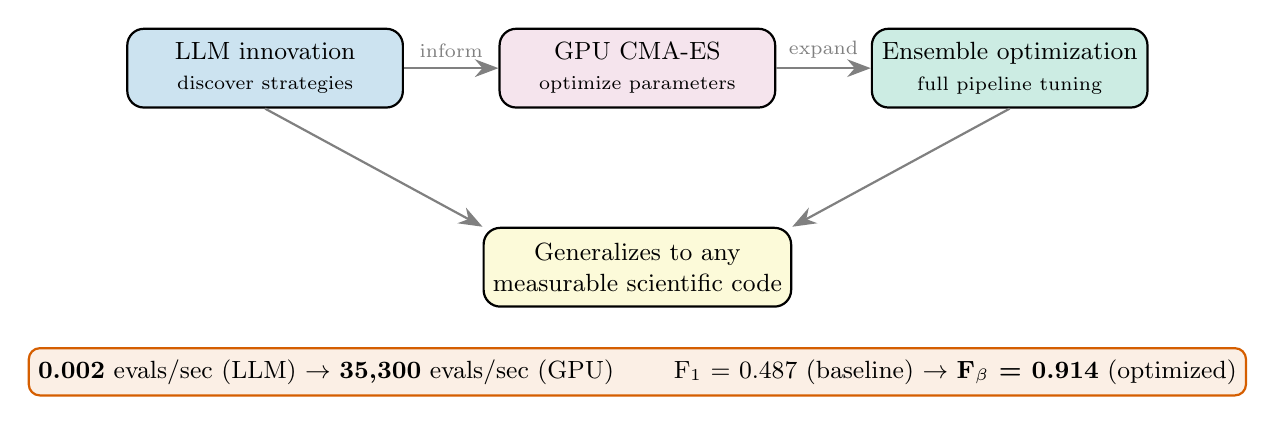
\begin{tikzpicture}[
    node distance=0.6cm,
    box/.style={draw, rounded corners=6pt, minimum width=3.5cm,
                minimum height=1.0cm, font=\small, align=center, thick},
    arr/.style={-{Stealth[length=3mm]}, thick, gray}
  ]
    \node[box, fill=cbBlue!20] (llm) {LLM innovation\\{\scriptsize discover strategies}};
    \node[box, fill=cbPurple!20, right=1.2cm of llm] (cma)
      {GPU CMA-ES\\{\scriptsize optimize parameters}};
    \node[box, fill=cbGreen!20, right=1.2cm of cma] (ensemble)
      {Ensemble optimization\\{\scriptsize full pipeline tuning}};

    \draw[arr] (llm) -- node[above, font=\scriptsize] {inform} (cma);
    \draw[arr] (cma) -- node[above, font=\scriptsize] {expand} (ensemble);

    % Applications below
    \node[box, fill=cbYellow!20, below=1.5cm of cma] (apps)
      {Generalizes to any\\measurable scientific code};

    \draw[arr] ($(llm.south)+(0,0)$) -- (apps.north west);
    \draw[arr] (ensemble.south) -- (apps.north east);

    % Performance banner
    \node[draw=cbOrange, thick, rounded corners, fill=cbOrange!10,
          font=\small, minimum width=12cm, minimum height=0.6cm,
          below=0.5cm of apps] (perf)
      {\textbf{0.002} evals/sec (LLM) $\to$ \textbf{35{,}300} evals/sec (GPU)
       ~~~~~
       F$_1$ = 0.487 (baseline) $\to$ \textbf{F$_\beta$ = 0.914} (optimized)};
  \end{tikzpicture}

  \vspace{0.5em}
  \begin{columns}[T]
    \begin{column}{0.30\textwidth}
      \centering
      \textbf{LLMs innovate}\\
      {\small Physics-grounded\\strategy discovery}
    \end{column}
    \begin{column}{0.30\textwidth}
      \centering
      \textbf{CMA-ES optimizes}\\
      {\small Exhaustive search\\of parameter space}
    \end{column}
    \begin{column}{0.30\textwidth}
      \centering
      \textbf{GPUs enable}\\
      {\small 7 orders of magnitude\\throughput gain}
    \end{column}
  \end{columns}
\note{
  The three pillars of this framework are LLM-driven innovation, CMA-ES
  numerical optimization, and GPU-accelerated evaluation. LLMs discover
  what to optimize. CMA-ES finds the optimal values. GPUs make the search
  tractable. Together they enable a pipeline that generalizes to any
  scientific code with a measurable fitness function. The headline numbers:
  7 orders of magnitude speedup in evaluation throughput, and F-beta from
  0.487 baseline to 0.914 optimized.
}
\end{frame}

% ----------------------------------------------------------
% SLIDE 19: Conclusions
% ----------------------------------------------------------
\begin{frame}{Conclusions}
  \begin{enumerate}
    \item Three-phase optimization progressively improved CF-LIBS element identification:\\
          LLM code evolution $\to$ GPU CMA-ES $\to$ GPU Sep\_CMA\_ES

    \vspace{0.3em}
    \item Final result: \alert{F$_\beta$(0.5) = 0.914} on 74 real mineral spectra\\
          {\small (from 0.487 baseline, \alert{+88\%} improvement; surpasses hand-tuned hybrid at 0.654)}

    \vspace{0.3em}
    \item LLMs discovered \textbf{9 physically interpretable} strategies\\
          that informed the CMA-ES parameter space design

    \vspace{0.3em}
    \item \textbf{7 orders of magnitude} speedup: 0.002 $\to$ 35{,}300 evals/sec

    \vspace{0.3em}
    \item Optimized parameters are \textbf{physically interpretable}:\\
          NNLS dominates, Mn/Na suppressed, SNR gate at 9.5

    \vspace{0.3em}
    \item Framework \textbf{generalizes} to any measurable scientific code optimization
  \end{enumerate}
\note{
  To summarize: we conducted a three-phase optimization campaign for CF-LIBS
  element identification. The final result is F-beta of 0.914 on real spectra,
  an 88 percent improvement over baseline and far surpassing the best hand-tuned
  approach. LLMs contributed physically interpretable strategy discoveries.
  GPU-accelerated CMA-ES delivered a 7-order-of-magnitude speedup. The optimized
  parameters are physically meaningful --- NNLS dominates, manganese and sodium
  are suppressed, and a strict SNR gate ensures reliable identification.
  The framework generalizes to any scientific code optimization problem.
}
\end{frame}

% ----------------------------------------------------------
% SLIDE 20: Thank You
% ----------------------------------------------------------
\begin{frame}[standout]
  Thank you

  \vspace{1em}
  {\large Questions?}

  \vspace{1em}
  {\normalsize F$_\beta$(0.5) = \textbf{0.914} ~~~ 7 orders of magnitude faster}
\note{
  Thank you for your attention. I am happy to take questions about the
  optimization framework, the spectroscopic details, or the LLM versus
  CMA-ES comparison.
}
\end{frame}

% ============================================================
% BACKUP SLIDES
% ============================================================
\appendix

% ----------------------------------------------------------
% BACKUP 1: MAP-Elites Detail
% ----------------------------------------------------------
\begin{frame}{Backup: MAP-Elites Quality-Diversity Search}
  \begin{columns}[T]
    \begin{column}{0.50\textwidth}
      \textbf{Quality-diversity algorithm}\\
      {\small (Mouret \& Clune, 2015)}

      \vspace{0.5em}
      \begin{itemize}
        \item Maintains archive of \emph{diverse, high-performing} solutions
        \item 2D behavior space: F$_1 \times$ Precision
        \item CVT tessellation with \alert{50 centroids}
        \item Each cell stores the best solution for that region
      \end{itemize}

      \vspace{0.5em}
      \textbf{Key advantage:}\\
      Discovers a \emph{Pareto front} of strategies,\\
      not a single optimum
    \end{column}
    \begin{column}{0.47\textwidth}
      \centering
      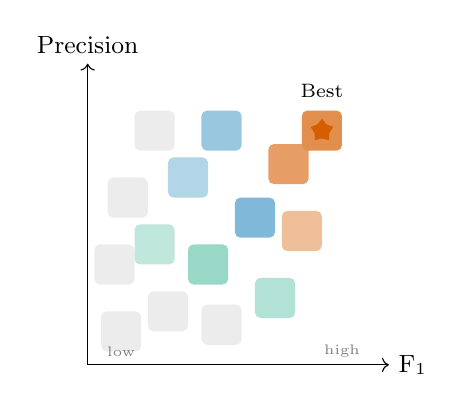
\begin{tikzpicture}[scale=0.85]
        % Axes
        \draw[->] (0,0) -- (4.5,0) node[right, font=\small] {F$_1$};
        \draw[->] (0,0) -- (0,4.5) node[above, font=\small] {Precision};
        % Grid cells (CVT-like)
        \foreach \x/\y/\c in {
          0.5/0.5/gray!15, 1.2/0.8/gray!15, 2.0/0.6/gray!15,
          0.4/1.5/gray!15, 1.0/1.8/cbGreen!25, 1.8/1.5/cbGreen!40,
          0.6/2.5/gray!15, 1.5/2.8/cbBlue!30, 2.5/2.2/cbBlue!50,
          2.8/1.0/cbGreen!30, 3.2/2.0/cbOrange!40, 3.0/3.0/cbOrange!60,
          3.5/3.5/cbOrange!70, 2.0/3.5/cbBlue!40, 1.0/3.5/gray!15
        }{
          \fill[\c, rounded corners=2pt] (\x-0.3,\y-0.3) rectangle (\x+0.3,\y+0.3);
        }
        % Star for best
        \node[star, star points=5, fill=cbOrange, inner sep=2pt] at (3.5,3.5) {};
        % Labels
        \node[font=\tiny, text=gray] at (0.5,0.2) {low};
        \node[font=\tiny, text=gray] at (3.8,0.2) {high};
        \node[font=\scriptsize] at (3.5,4.1) {\alert{Best}};
      \end{tikzpicture}

      {\scriptsize Colored cells = occupied; intensity = fitness}
    \end{column}
  \end{columns}
\note{
  MAP-Elites is a quality-diversity algorithm that maintains an archive
  of diverse, high-performing solutions. We tessellate a 2D behavior space
  of F1 score versus precision with 50 CVT centroids. Each cell keeps
  the best solution found for that region. This gives us a Pareto front
  of strategies, not just a single optimum.
}
\end{frame}

% ----------------------------------------------------------
% BACKUP 2: MAP-Elites vs Single-Objective
% ----------------------------------------------------------
\begin{frame}{Backup: MAP-Elites vs Single-Objective}
  \begin{columns}[T]
    \begin{column}{0.48\textwidth}
      \textbf{Why not just maximize F$_1$?}
      \begin{itemize}
        \item A single optimum misses the precision--recall tradeoff
        \item F$_1 = 0.595$ at P=0.61 is very different from F$_1 = 0.595$ at P=0.655
        \item Applications have different needs
      \end{itemize}
    \end{column}
    \begin{column}{0.48\textwidth}
      \textbf{MAP-Elites populates the behavior space:}
      \begin{itemize}
        \item \textcolor{cbGreen}{Planetary science:}\\
              P=0.658, 41 FP (conservative)
        \item \textcolor{cbBlue}{Industrial monitoring:}\\
              R=0.653, 100 FP (sensitive)
        \item \textcolor{cbOrange}{General analysis:}\\
              F$_1$=0.595, 62 FP (balanced)
      \end{itemize}

      \vspace{0.3em}
      The user chooses their operating point \emph{after} optimization
    \end{column}
  \end{columns}
\note{
  A single-objective optimizer would find one point on the precision-recall
  curve. MAP-Elites populates the entire tradeoff space, letting the user
  choose their operating point post-hoc.
}
\end{frame}

% ----------------------------------------------------------
% BACKUP 3: Exploration Schedule
% ----------------------------------------------------------
\begin{frame}{Backup: Adaptive Exploration Schedule}
  \begin{columns}[T]
    \begin{column}{0.48\textwidth}
      \textbf{Exploration rate} controls how often the exploration
      (high-temperature) ensemble is chosen vs the exploitation
      (low-temperature) ensemble.

      \vspace{0.5em}
      \begin{table}
        \footnotesize
        \begin{tabular}{@{}ll@{}}
          \toprule
          Parameter & Value \\
          \midrule
          Initial rate & 0.25 \\
          Range & 0.15 -- 0.50 \\
          Increase factor & 1.05 \\
          Decrease factor & 0.95 \\
          Plateau threshold & 5 epochs \\
          \bottomrule
        \end{tabular}
      \end{table}
    \end{column}
    \begin{column}{0.48\textwidth}
      \textbf{Adaptation logic:}
      \begin{itemize}
        \item No improvement for 5 epochs $\to$ increase exploration
              (factor $\times 1.05$)
        \item New best found $\to$ decrease exploration
              (factor $\times 0.95$)
        \item Clamped to $[0.15, 0.50]$
      \end{itemize}

      \vspace{0.5em}
      \textbf{Intuition:}\\
      When stuck, explore more.\\
      When improving, exploit more.
    \end{column}
  \end{columns}
\note{
  The exploration rate adapts during the run. Starting at 0.25, it increases
  by a factor of 1.05 after 5 epochs without improvement, and decreases
  by 0.95 when a new best is found.
}
\end{frame}

% ----------------------------------------------------------
% BACKUP 4: Full Baseline Comparison (updated)
% ----------------------------------------------------------
\begin{frame}{Backup: Full Optimization Progression}
  {\small
  \begin{table}
    \centering
    \begin{tabular}{@{}rlcccl@{}}
      \toprule
      Rank & Method & P & R & F$_\beta$(0.5) & Notes \\
      \midrule
      \rowcolor{cbGreen!15}
      1 & \textbf{Sep\_CMA\_ES 101p} & --- & --- & \textbf{0.914} & \textbf{5-algo ensemble, GPU} \\
      2 & Hybrid hand-tuned & 0.604 & 0.713 & 0.654* & 2 identifiers \\
      3 & Evolved ALIAS-only & 0.610 & 0.581 & 0.595* & LLM-discovered, 1 ident. \\
      4 & ALIAS (benchmark) & 0.505 & 0.629 & 0.560* & Hand-tuned baseline \\
      5 & CMA-ES 41p & --- & --- & 0.551 & Single-algo global opt. \\
      6 & Voigt + ALIAS & 0.488 & 0.623 & 0.547* & Deconvolution \\
      7 & Forward model & 0.369 & 0.796 & 0.505* & High recall \\
      8 & ALIAS (combiner) & 0.396 & 0.635 & 0.487* & Optimization seed \\
      9 & Spectral NNLS & 0.293 & 0.940 & 0.447* & High recall, low P \\
      \bottomrule
    \end{tabular}
  \end{table}
  }

  \vspace{0.3em}
  {\footnotesize *F$_1$ metric (not directly comparable to F$_\beta$); shown for reference.
   Sep\_CMA\_ES F$_\beta$=0.914 surpasses all methods by a wide margin.}
\note{
  Placing all results in context: the Sep-CMA-ES 101-parameter optimization
  achieves F-beta of 0.914, dramatically surpassing the best hand-tuned hybrid
  at F1 of 0.654. Note the metric difference: earlier methods were evaluated
  on F1 while CMA-ES phases used F-beta with precision weighting. Even accounting
  for this, the improvement is massive. The evolved ALIAS-only combiner from
  Phase 1 sits at F1 of 0.595, which informed the CMA-ES parameter design.
}
\end{frame}

% ----------------------------------------------------------
% BACKUP 5: Recall Bias Analysis (NEW)
% ----------------------------------------------------------
\begin{frame}{Backup: LLM Recall Bias in Code Generation}
  \begin{columns}[T]
    \begin{column}{0.48\textwidth}
      \textbf{Observed pattern across 3 CodeEvolve runs:}

      \vspace{0.3em}
      {\small
      \begin{table}
        \begin{tabular}{@{}lccc@{}}
          \toprule
          Run & Best P & Best R & Bias \\
          \midrule
          1 (F$_1$) & 0.610 & 0.581 & Moderate \\
          2a (F$_1$) & 0.425 & 0.743 & \alert{Strong R} \\
          2b (F$_\beta$) & 0.460 & 0.557 & Corrected \\
          \bottomrule
        \end{tabular}
      \end{table}
      }

      \vspace{0.3em}
      \textbf{F$_1$ asymmetry:}\\
      {\small Improving R from 0.62$\to$0.74 gains\\
       more F$_1$ than improving P from 0.41$\to$0.50.\\
       LLMs follow the steepest gradient.}
    \end{column}
    \begin{column}{0.48\textwidth}
      \textbf{Hypothesized causes:}
      \begin{enumerate}
        \item Training data bias: more\\
              ``if X exists'' than ``if X doesn't''
        \item Easier to lower thresholds\\
              than add rejection logic
        \item Asymmetric error visibility:\\
              FN feels worse than FP to LLMs
      \end{enumerate}

      \vspace{0.5em}
      \textbf{Mitigation:}
      \begin{itemize}
        \item F$_\beta$(0.5): weights P $2\times$ over R
        \item System prompt precision hints
        \item Hard gates (P $>$ 0.20)
        \item Ultimately: \emph{use CMA-ES}\\
              (no cognitive bias)
      \end{itemize}
    \end{column}
  \end{columns}
\note{
  The recall bias was a consistent pattern across all three CodeEvolve runs.
  Run 2a showed it most dramatically: recall shot to 0.743 while precision
  fell to 0.425. The F1 metric creates an asymmetric gradient favoring recall.
  We hypothesize three causes: training data bias, the ease of lowering
  versus raising thresholds, and asymmetric error visibility. F-beta with
  precision weighting and system prompt hints helped but didn't fully solve it.
  Ultimately, switching to CMA-ES eliminated the problem entirely ---
  numerical optimizers have no cognitive biases.
}
\end{frame}

% ----------------------------------------------------------
% BACKUP 6: CMA-ES Technical Detail (NEW)
% ----------------------------------------------------------
\begin{frame}{Backup: CMA-ES Technical Details}
  \begin{columns}[T]
    \begin{column}{0.48\textwidth}
      \textbf{Covariance Matrix Adaptation ES}
      \begin{itemize}
        \item Derivative-free, population-based
        \item Adapts search distribution\\
              covariance $\to$ learns correlations
        \item Sep\_CMA\_ES: diagonal covariance\\
              {\scriptsize (avoids $O(n^2)$ matrix ops for $n=101$)}
        \item evosax: JAX-based, GPU-native
      \end{itemize}

      \vspace{0.5em}
      \textbf{V100S GPU setup:}
      \begin{itemize}
        \item 32 GB HBM2, 900 GB/s bandwidth
        \item Fitness evaluation fully vectorized\\
              via JAX (no Python loops)
        \item 4{,}096 candidates evaluated in\\
              parallel per generation
      \end{itemize}
    \end{column}
    \begin{column}{0.48\textwidth}
      \textbf{Why Sep\_CMA\_ES for 101-dim?}
      \begin{itemize}
        \item Full CMA-ES: $O(n^2)$ covariance\\
              ($101^2 = 10{,}201$ entries)
        \item cuSolver eigendecomposition\\
              fails on V100S Volta architecture
        \item Sep\_CMA\_ES: $O(n)$ diagonal\\
              covariance, GPU-safe
        \item Trade: loses inter-parameter\\
              correlation learning
      \end{itemize}

      \vspace{0.5em}
      \textbf{Cache design:}
      \begin{itemize}
        \item All 5 algorithms pre-computed\\
              on all 74 spectra
        \item JAX arrays: (74, 22, 5--8) per algo
        \item Fitness = pure array operations\\
              (no I/O during optimization)
      \end{itemize}
    \end{column}
  \end{columns}
\note{
  CMA-ES adapts the covariance matrix of a multivariate Gaussian search
  distribution, learning correlations between parameters. For 101 dimensions,
  full CMA-ES requires a 10,201-entry covariance matrix, and the eigendecomposition
  fails on V100S due to a cuSolver bug. Sep-CMA-ES uses a diagonal covariance,
  trading inter-parameter correlation learning for GPU compatibility.
  The cache pre-computes all five algorithm outputs, so the fitness function
  is pure array operations with no I/O. This enables 45,000 evaluations
  per second on a single V100S.
}
\end{frame}

% ----------------------------------------------------------
% BACKUP 7: Per-Island Performance (original, condensed)
% ----------------------------------------------------------
\begin{frame}{Backup: Phase 1 Island Performance}
  \begin{columns}[T]
    \begin{column}{0.52\textwidth}
      {\small
      \begin{table}
        \centering
        \begin{tabular}{@{}ccccl@{}}
          \toprule
          Island & Best F$_1$ & Epoch & Evals & Notes \\
          \midrule
          0 & 0.506 & 13 & 12 & Stuck near baseline \\
          1 & 0.543 & 1 & 10 & Early win, stalled \\
          \rowcolor{cbGreen!15}
          2 & \alert{0.595} & 9 & 13 & Dominant \\
          \bottomrule
        \end{tabular}
      \end{table}
      }

      \vspace{0.3em}
      \textbf{Island 2} found multiple good solutions\\
      across different archive cells
    \end{column}
    \begin{column}{0.45\textwidth}
      \textbf{Observations:}
      \begin{itemize}
        \item Significant variance across islands
        \item Island 0 never escaped baseline
        \item Migration sent weak solutions\\
              to strong islands (wasted)
        \item Initial seed + first model\\
              strongly determines trajectory
      \end{itemize}
    \end{column}
  \end{columns}
\note{
  Performance varied significantly across islands. Island 2 was dominant.
  Migration was too infrequent to help weak islands. The initial random seed
  plus first model selection strongly determined island trajectory.
}
\end{frame}

% ============================================================
\end{document}
